\documentclass[a4paper]{article}

\usepackage[utf8]{inputenc}
\usepackage{indentfirst}
\usepackage{polski}
\usepackage{graphicx}
\usepackage{xcolor}
\usepackage{geometry}
\usepackage{minted}
\usepackage{float}


\newcommand\tab[1][1cm]{\hspace*{#1}}

\title{\textbf{Zraszacze Ogrodowe}}
\author{Jakub Grenda\\ Kamil Sztandur\\ Robert Odrowąż-Sypniewski}
\date{15/04/2020}
\begin{document}
\maketitle

\section{Cel Projektu}
Celem naszego projektu było stworzenie programu, który pomagałby ogrodnikom w optymalnym rozstawieniu zraszaczy ogrodowych na terenie swojego trawnika. Program ten uwzględnia różne kształty terenu oraz obecne przeszkody na nim. Jego zadaniem jest rozstawienie odpowiedniej liczby czterech rodzajów zraszaczy ogrodowych tak, aby trawnik był podlany równomiernie na całej powierzchni. Program informuje użytkownika o ilości rozstawionych zraszaczy, ich koordynatach (oraz typach i kierunkach na konkretnych współrzędnych), średni stopień podlania całego trawnika oraz odchylenie standardowe od niego.
\newline

Użytkownik wprowadza do programu kształt swojego trawnika oraz oczekiwaną liczbę cykli obrotów zraszaczy formie, którą opiszemy w dalszej części dokumentacji. Program odczytuje wprowadzone przez użytkownika dane i za pomocą trenowanego algorytmu rozstawia odpowiednio zraszacze. Pod koniec swojej pracy zapisuje stan trawnika do pliku typu png (\textit{Portable Network Graphics}), zawierającego heatmapę stopnia podlania poszczególnych fragmentów trawnika. Program generuje także plik .txt, w którym wypisana zostaje ilość rozstawionych zraszaczy, średnią arytmetyczną podlanego trawnika oraz odchylenie standardowe od średniej.

\section{Dane wejściowe programu}
Dla poprawnego działania programu należy go uruchomi w terminalu podając jeden argument wejściowy będący ścieżką do plika zawierającego liczbą cykli jaką mają wykonać zraszacze oraz kształt trawnika, na którym mają zostać one rozmieszczone. W pierwszej linii pliku określona jest liczba cykli, w kolejnych 40 liniach o zawierających 80 znaków danych oraz znak nowej linii określony jest kształt trawnika. Znaki danych to symbole '-' lub '*' gdzie '-' oznacza brak trawnika w danym punkcie natomiast '*' oznacza jego obecność. Każdy znak odpowiada kwadratowi o wymiarach 100x100 pixeli pliku wyjściowego png.

\newpage
\subsection*{Przykładowy plik wejściowy}
\begin{verbatim}
21
--------------------------------------------------------------------------------
--------------------------------------------------------------------------------
----****************************************************************------------
----****************************************************************------------
----****************************************************************------------
----****************************************************************------------
----****************************************************************------------
----****************************************************************------------
----****************--------****************--------****************------------
----****************--------****************--------****************------------
----****************--------****************--------****************------------
----****************--------****************--------****************------------
----****************--------****************--------****************------------
----****************--------****************--------****************------------
----************************************************************************----
----************************************************************************----
----************************************************************************----
----************************************************************************----
----************************************************************************----
----************************************************************************----
----****************--------****************************************------------
----****************--------****************************************------------
----****************--------****************************************------------
----****************--------****************************************------------
----****************--------****************************************------------
----****************--------****************************************------------
----************************************************************************----
----************************************************************************----
----************************************************************************----
----************************************************************************----
----************************************************************************----
----************************************************************************----
----****************--------************************--------****************----
----****************--------************************--------****************----
----****************--------************************--------****************----
----****************--------************************--------****************----
----****************--------************************--------****************----
----****************--------************************--------****************----
--------------------------------------------------------------------------------
--------------------------------------------------------------------------------
\end{verbatim}

\section{Przegląd sytuacji wyjątkowych opisywanych przez program.}
\subsection{Wejście}
\begin{enumerate}
    \item Użytkownik nie podaje żadnego argumentu.
          \begin{itemize}
              \item Program wyświetla użytkownikowi poprawną instrukcję wywołania programu help().
              \item Program przerywa pracę.
          \end{itemize}
    \item Użytkownik podaje jako argument nieistniejący plik.
          \begin{itemize}
              \item Program informuje użytkownika poprzez terminal o niepoprawnym podaniu pliku tekstowego.
              \item Program wyświetla użytkownikowi instrukcję help().
              \item Program przerywa pracę.
          \end{itemize}
    \item Użytkownik podaje jako argument plik niezawierający liczby cykli w pierwszej linijce.
          \begin{itemize}
              \item Program wyświetla użytkownikowi poprawną instrukcję wywołania programu help().
              \item Program przerywa pracę.
          \end{itemize}
    \item Użytkownik podaje jako argument plik z ujemną liczbą cykli.
          \begin{itemize}
              \item Program wyświetla użytkownikowi poprawną instrukcję wywołania programu help().
              \item Program przerywa pracę.
          \end{itemize}
\end{enumerate}

\section{Algorytm rozmieszczający zraszacze}
Działanie algorytmu rozpoczyna się od znalezienia i zaznaczenia w pomocniczej tablicy \mintinline[breaklines]{c}{int** edges} krawędzi trawnika. Dla zwiększenia wydajności algorytm na tym etapie operuje na danych o rozdzielczości pliku wejściowego tj. 80x40.

\begin{figure}[H]
    \includegraphics[width=10cm]{edges.png}
    \centering
    \caption{Odnalezione krawędzie trawnika}
\end{figure}

Po odnalezieniu krawędzie algorytm znajduje rogi o kącie \(90^{\circ}\) i umieszcza w nich zraszacze o takim zakresie podlewania. Następnie w na rogach o kącie \(270^{\circ}\) umieszczane są odpowiednie zraszacze. Jako ostatnie rozstawiane są zraszacze \(180^{\circ}\) wzdłuż prostych krawędzi trawnika.

\begin{figure}[H]
    \includegraphics[width=10cm]{edge_sprinklers.png}
    \centering
    \caption{Trawnik po rozmieszczeniu krawędziowych zraszaczy}
\end{figure}

Następnie we wszystkich dotąd niepodlanych punktach ustawiane są zraszacze o zakresie pełnego okręgu rozpoczynając od lewego górnego rogu.

\begin{figure}[H]
    \includegraphics[width=10cm]{all_sprinklers.png}
    \centering
    \caption{Trawnik po wszystkich zraszaczy}
\end{figure}

W trakcie działania algorytmu wyniki zapisywane są do wektora zawierającego listę zraszaczy oraz stopień podlania trawnika renderowany jest do tablicy, na podstawie której eksportowany jest wyjściowy plik png.

\section{Opis funkcji udostępnianych przez program}

Program dysponuje wachlarzem funkcji odpowiedzialnych za obsługę plików png, txt, list liniowych, tablic dwuwymiarowych oraz funkcji matematycznych i debugujących.

\subsection{Lista zraszaczy}
\begin{enumerate}
    \item \mintinline[breaklines]{c}{location *set_new(location *tab, int x, int y, SprinklerType type, int direction, int *spr_size, int *spr_count)} - funkcja dodając zraszacz do listy na podastawie której generowany jest plik wyjściowy txt zawierający listę pozycji oraz typów zraszaczy.
    \item \mintinline[breaklines]{c}{location *increase(location *tab, int *spr_size)} - funkcja powiększająca dwukrotnie pojemność listy zraszaczy w razie przepełnienia.
\end{enumerate}

\subsection{Rysowanie zraszaczy po tablicy 2D trawnika}
\begin{enumerate}
    \item \mintinline[breaklines]{c}{void draw_circle(int **tab, int x, int y, SprinklerType type, Direction direction, int add_value)} - główna funkcja uruchamiająca dany zraszacz. Jej zadaniem jest podlanie znajdującego się w jego zasięgu terenu na podstawie koordynatów oraz iloczynu kartezjańskiego typu i kierunku zraszacza \textit{(Rysunek 1.)}. Funkcja przyjmuje dodatkowo argument \mintinline[breaklines]{c}{add_value}, który zgodnie ze swoją nazwą wskazuje o ile należy podlać wszystkie komórki w zasięgu zraszacza. Program w głównej funkcji liczy tę wartość na podstawie wskazanej przez użytkownika liczby cykli oraz czasu potrzebnego do obrotu danego typu zraszacza (np. ćwiartka w ciągu 1 cyklu obróci się 4 razy, a pełny kołowy zraszacz tylko raz).
          \begin{figure}[H]
              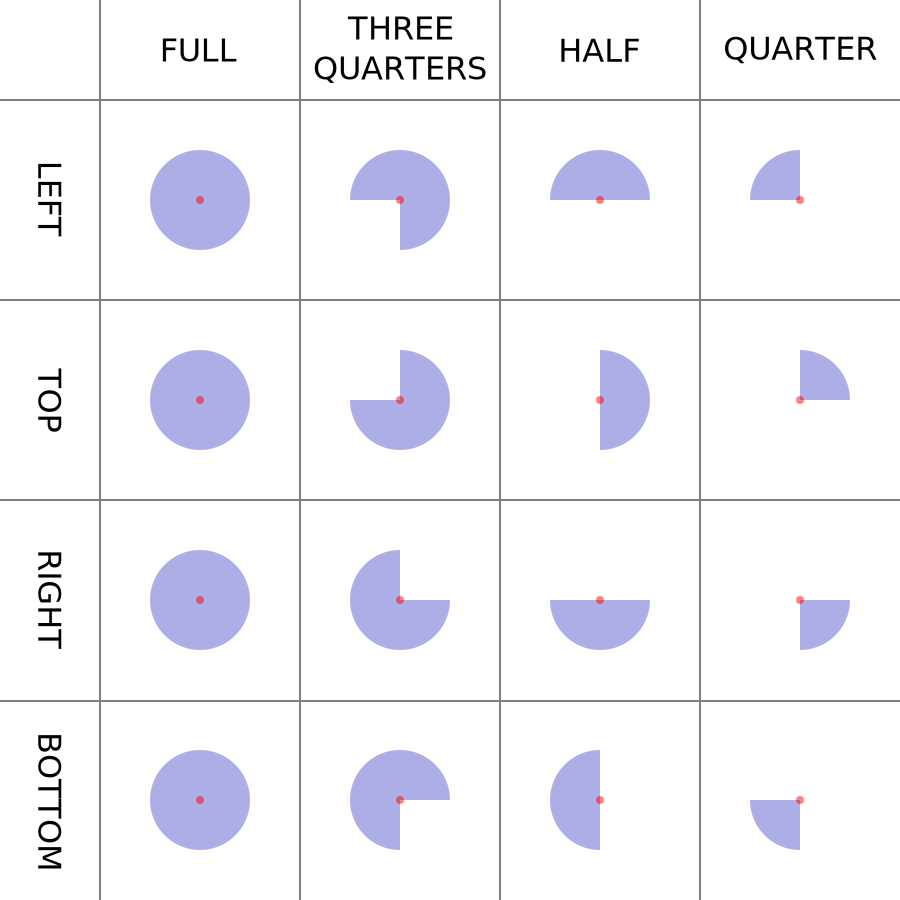
\includegraphics[width=10cm]{sprinklers.png}
              \centering
              \caption{\textit{Tabelka zraszaczy ze względu na iloczyn kartezjański ich typu i kierunku.}}
          \end{figure}
\end{enumerate}

\subsection{Tworzenie obrazka png}
\begin{enumerate}
    \item \mintinline[breaklines]{c}{static pixel_t *pixel_at(bitmap_t *bitmap, int r, int c)} - funkcja wskazująca bieżąco edytowany pixel na obrazku png
    \item \mintinline[breaklines]{c}{static int save_png_to_file(bitmap_t *bitmap, const char *path)} - funkcja eksportująca pokolorowaną tablicę 2D do pliku PNG
    \item \mintinline[breaklines]{c}{int make_png(int **tab, int height, int width, int count, char *filename, double spr_average, double spr_deviation)} - funkcja główna modułu eksportującego tablicę do pliku png.
\end{enumerate}

Każdy pixel trawnika jest kolorowany w oparciu o wartość odpowiadającej mu komórki w tablicy 2D. Sposób kolorowania jest zależny od wyliczonej średniej arytmetycznej oraz odchylenia standardowego \textit{(Rysunek 2.)}.

\begin{figure}[H]
    \includegraphics[width=10cm]{kolory}
    \centering
    \caption{\textit{Metoda kolorowania komórek}}
\end{figure}

\begin{itemize}
    \item Wartości spomiędzy przedziału (E(x) – D(x), E(x) + D(x)) są gradientem zieleni (jasne od dolnej granicy i ciemne z górnej granicy).
    \item Wartości poniżej dolnej granicy są koloru zgniło-żółtego ( 185, 140, 30 ) i oznaczają niedostatecznie podlane komórki w porównaniu do całości.
    \item Wartości powyżej górnej granicy są koloru czerwonego (220, 30, 30) i oznaczają zbytnio podlane komórki w porównaniu do całości.
\end{itemize}

\begin{figure}[H]
    \includegraphics[width=10cm]{all_sprinklers.png}
    \centering
    \caption{Przykładowy wynik renderowania}
\end{figure}
\newpage
\subsection{Tworzenie pliku txt:}
\begin{enumerate}
    \item \mintinline[breaklines]{c}{void make_txt(location *sprinklers, int count, char *filename,
    double spr_average, double spr_deviation, int spr_count)} - funkcja wypisująca listę zraszaczy, ich ilość, średnią arytmetyczną poziomu nawodnienia oraz odchylenie standardowe od średniej do pliku txt.
\end{enumerate}

\subsection*{Przykładowy plik wyjściowy}
\begin{figure}[H]
	\includegraphics[width=10cm]{koordynaty.png}
	\centering
\end{figure}

\subsection{Obliczanie średniej oraz odchylenia standardowego:}


\begin{enumerate}
    \item \mintinline[breaklines]{c}{average()} - funkcja zwracająca średnią arytmetyczną wartości na tablicy posługująca się 	wzorem:
          \[E_{(x)} = \frac{\sum_{i=1}^n x_i}{n}\]
          gdzie $x_i$ to kolejne wartości komórek tablicy, a $n$ to liczba wszystkich komórek.

    \item \mintinline[breaklines]{c}{std_deviation()} - funkcja zwracająca odchylenie standardowe na tablicy posługująca się 	wzorem:
          \[D(x) = \sqrt{\frac{\sum_{i=1}^n (x_i - E_{(x)})^2 }{n}}\]
          gdzie \(E_{(x)}\) to średnia arytmetyczna.
\end{enumerate}


\subsection{Pomoc:}

\begin{enumerate}
    \item help() - funkcja wyświetlająca instrukcję prawidłowego wywoływania programu.
\end{enumerate}



\subsection{Kolorowanie:}
\begin{enumerate}
    \item Wartość podlania komórki wykracza ponad 255 (maksymalna wartość składowej RGB).
          \begin{itemize}
              \item Nie jest to żadnym problemem, ponieważ program opiera się na średniej arytmetycznej i odchyleniu standardowym. Gradient pomiędzy górną granicą, a dolną ma zabarwienie proporcjonalne. Wartość komórek zostaje przeskalowana względem tego przedziału.
          \end{itemize}
    \item Średnia arytmetyczna jest mniejsza niż odchylenie standardowe (wartości dolnego 		    przedziału wchodzą na minus).
          \begin{itemize}
              \item Program jako dolną granicę przyjmuje 0.
          \end{itemize}
\end{enumerate}
\end{document}
